\begin{frame}{Stående jagthunde}

\vspace{1em}

\begin{columns}[c] % c = center vertically

\column{0.05\textwidth} % Venstre margin

\column{0.7\textwidth} % Midten: Bullets

\small

\raggedright

\begin{itemize}

\itemsep0.6em % Justér afstand mellem bullets

\item Udfører et \textbf{langt søg} i terrænet.
\item God til jagt i områder med \textbf{stor vildtspredning}.
\item Deres kendetegn er at \textbf{tage stand} for fuglevildt (pege). 
\item Opdeles primært i to typer: \textbf{Engelsk} (f.eks. Pointer, Setter) og \textbf{Kontinental} (f.eks. Ruhåret Hønsehund).
\item Anvendes til jagt på hønsefugle - jagtformen er aftagende.
\item \textbf{Racer}: Hønsehunde, Pointere, Settere, Wizla, Münsterländere, Breton, Weimaraner

\end{itemize}

\column{0.25\textwidth} % Højre: Ikon

\centering

\vspace{0pt}

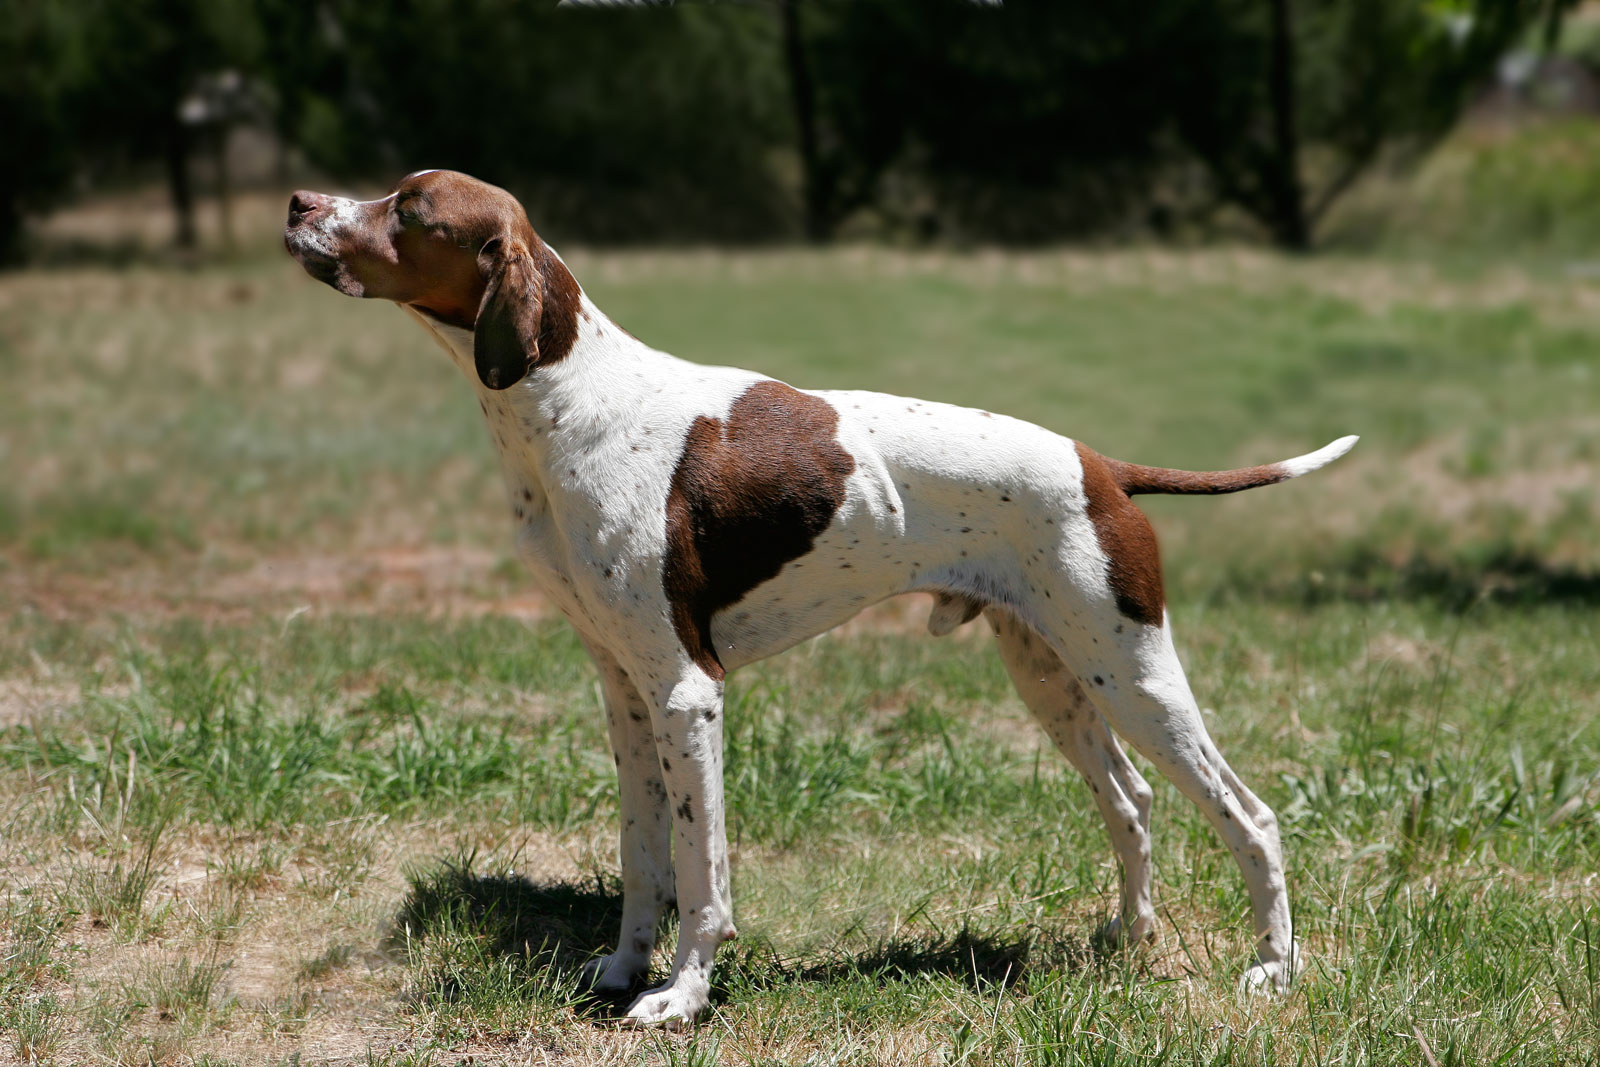
\includegraphics[width=0.9\linewidth]{Billeder/Jagthunde/staaende/English_pointer.jpg} % Ikon af stående hund

\end{columns}

\end{frame}